\documentclass[american]{scrartcl}
    \usepackage{babel}
    \usepackage[utf8]{inputenc} 
    \usepackage{csquotes}
    \usepackage{amsmath}
    \usepackage{amssymb}
    \usepackage{graphicx}   
    \usepackage{mathtools}
    \usepackage{tikz}
    \usepackage{booktabs}
    \usepackage{color}
    \usepackage{bm}
    \usepackage{hyperref}
    
    
    \setlength{\parindent}{0em}
    \setlength{\parskip}{0.5em}

    \title{Exercises recipe}
    \subtitle{Evolutionary Game Theory}

    \author{A. Fisherman}
    

% Commands
\newcommand{\set}[1]{\left\{#1\right\}}
\newcommand{\Real}{\mathbb{R}}
\newcommand{\abs}[1]{\left\lvert #1 \right\rvert}
\newcommand{\E}{\mathbb{E}}

% chart
\usetikzlibrary{arrows.meta,
                calc, chains,
                quotes,
                positioning,
                shapes.geometric}


\begin{document}

% Title
\maketitle

\section{Weibull dynamics}

\subsection{Steps to solve}

You are given a matrix $\bm{P} \in \Real^{n\times n}$ which represents the payoffs.

\subsubsection{Utilities}

Given a vector $\bm{x} = \begin{pmatrix}
        x_1 & x_2 & \ldots & x_3
    \end{pmatrix}^T$ and $\bm{y}$ compute,

\begin{equation}
    u(\bm{x}, \bm{y}) = \bm{x} \bm{P} \bm{y}
\end{equation}

Note that you can just set $\bm{x} \mapsto \bm{y}$ or vice-versa to get all of the utilities combinations.

\subsubsection{Nash equilibria}

Compute the Nash Equilibria of the symmetric game $(\bm{P}, \bm{P^T})$. Remember the mixed strategy. To find the mixed strategy you have to look at every combination of
\begin{equation}
    \bm{x} \in \left\{ \begin{pmatrix}
        \alpha \\ \beta \\ 1 - \alpha - \beta
    \end{pmatrix}, \begin{pmatrix}
        \alpha \\ 1 - \alpha \\ 0
    \end{pmatrix}, \begin{pmatrix}
        \alpha \\ 0 \\ 1 - \alpha
    \end{pmatrix}, \begin{pmatrix}
        0 \\ \alpha \\ 1 - \alpha
    \end{pmatrix} \right\}
\end{equation}.

You can also use \href{https://cgi.csc.liv.ac.uk/~rahul/bimatrix_solver/}{the online Irs solver by Avis and Fukuda}. Make sure to

\begin{enumerate}
    \item Put $3 \ 3$ as dimensions on top
    \item Click \textbf{Symmetric} under \textbf{type of game}
    \item Input matrix $\bm{P}$
    \item Only pick the symmetric Nash equilibria
\end{enumerate}

\subsubsection{ESS and NSS}

Once you found the Nash equilibrium, for each one do,
\begin{center}
    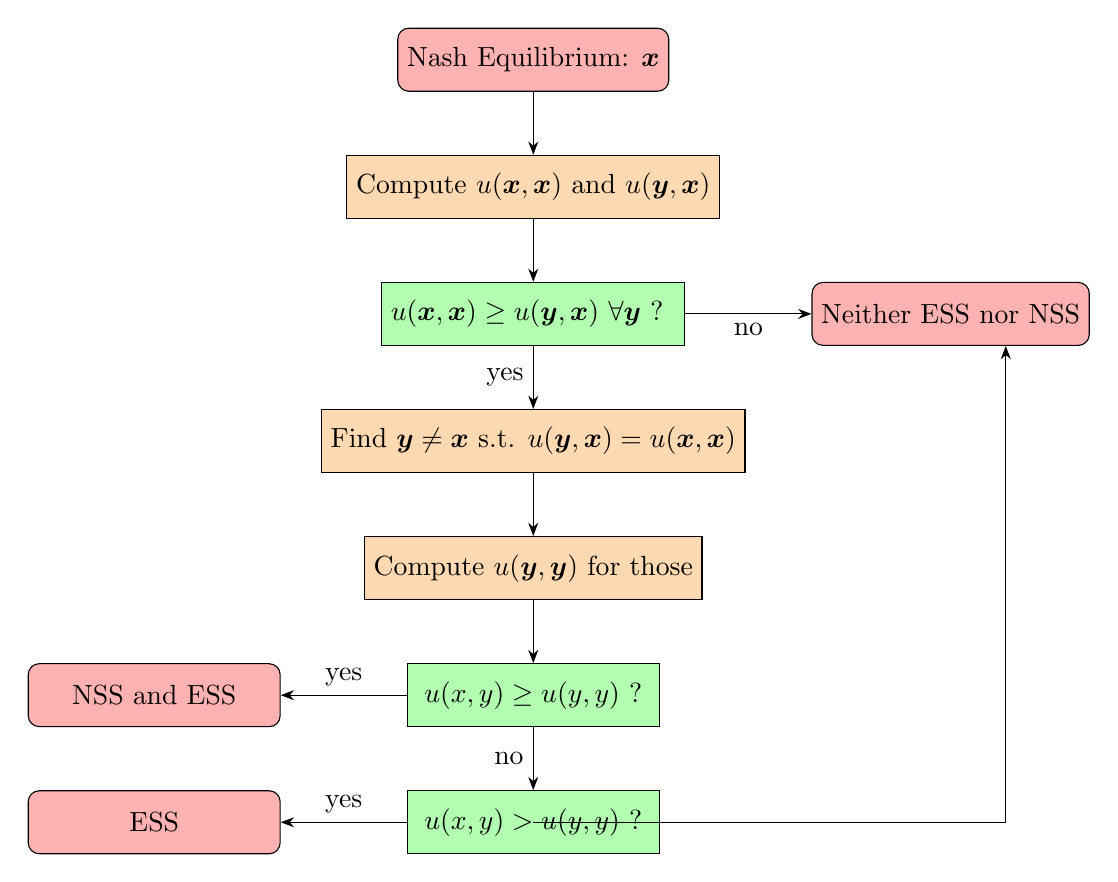
\begin{tikzpicture}[
            node distance = 8mm and 16mm,
            start chain = A going below,
            base/.style = {draw, minimum width=32mm, minimum height=8mm,
                    align=center, on chain=A},
            startstop/.style = {base, rectangle, rounded corners, fill=red!30},
            process/.style = {base, rectangle, fill=orange!30},
            decision/.style = {base, rectangle, fill=green!30},
            every edge quotes/.style = {auto=right}]

        \node [startstop]       {Nash Equilibrium: $\bm{x}$}; % A-1
        \node [process]         {Compute $u(\bm{x}, \bm{x})$ and $u(\bm{y}, \bm{x})$}; % A-2
        \node [decision]        {$u(\bm{x}, \bm{x}) \geq u(\bm{y}, \bm{x}) \ \forall \bm{y}$ ? }; % A-3
        \node [process]         {Find $\bm{y} \neq \bm{x}$ s.t. $u(\bm{y}, \bm{x}) = u(\bm{x}, \bm{x})$}; % A-4
        \node [process]         {Compute $u(\bm{y}, \bm{y})$ for those}; % A-5
        \node [decision]        {$u(x, y) \geq u(y, y)$ ?}; % A-6
        \node [decision]        {$u(x, y) > u(y, y)$ ?}; % A-7

        % Out
        \node [startstop,
            right =of A-3]      {Neither ESS nor NSS}; % A-8
        \node [startstop,
            left =of A-6]      {NSS and ESS}; % A-9
        \node [startstop,
            left =of A-7]      {ESS}; % A-10
        %%
        \draw [arrows=-Stealth]
        (A-1) edge  (A-2)
        (A-2) edge (A-3)
        (A-3) edge["yes"] (A-4)
        (A-3) edge["no"] (A-8)
        (A-4) edge (A-5)
        (A-5) edge (A-6)
        (A-6) edge["yes"] (A-9)
        (A-6) edge["no"] (A-7)
        (A-7) edge["yes"] (A-10)
        (A-7) |- ($(A-7.east)!0.!(A-8.south)$)
        -|([xshift=7mm] A-8.south);
    \end{tikzpicture}
\end{center}

\subsubsection{Replicator dynamics}

Let $\bm{e}^1 = \begin{pmatrix}
        1 & 0 & 0
    \end{pmatrix}$. The replicator dynamics are

\begin{equation}
    \dot{\bm{x}}_i = \left[ u(\bm{e}^i, \bm{x}) - u(\bm{x}, \bm{x}) \right] \cdot \bm{x}_i
\end{equation}

The main steps to find the dynamics are,

\begin{enumerate}
    \item Find fixed points $u(\bm{e}^i, \bm{x}) = u(\bm{x}, \bm{x})$
    \item Find dynamics on the boundaries, so set $\bm{x_j} = 0$ for all $j$
    \item Find dynamics on the bisector, like $\bm{x} = \begin{pmatrix}
                  \alpha & \alpha & 1 - 2\cdot \alpha
              \end{pmatrix}$ with $\alpha < 1 / 2$
\end{enumerate}

\subsection{Example, ex. 14}

Given

\begin{equation}
    \bm{P} = \begin{pmatrix}
        1 & 0 & 0 \\
        0 & 1 & 1 \\
        0 & 1 & 0
    \end{pmatrix}
\end{equation}

\subsubsection{Utilities}

\begin{equation}
    \begin{split}
        u(\bm{x}, \bm{y}) &= x_1 \cdot y_1 + x_2 \cdot \overbrace{(y_2 + y_3)}^{1 - y_1} + \overbrace{(1 - x_1 - x_2)}^{x_3} \cdot y_2 \\
        (\bm{y} \mapsto \bm{x}), \ u(\bm{x}, \bm{x}) &= x_1^2  + x_2 \cdot (1 - x_1) + x_3 \cdot x_2
    \end{split}
\end{equation}

\subsubsection{Nash equilibria}

We get

\includegraphics[width=\textwidth]{images/ne_out.PNG}

We only want the symmetric ones so rows 1, 3, and 5, namely,

\begin{equation}
    NE = \set{ (1, 0, 0), (0, 1, 0), (1 / 2, 1/2, 0) }
\end{equation}

\subsubsection{ESS and NSS}

The third one,


\begin{center}
    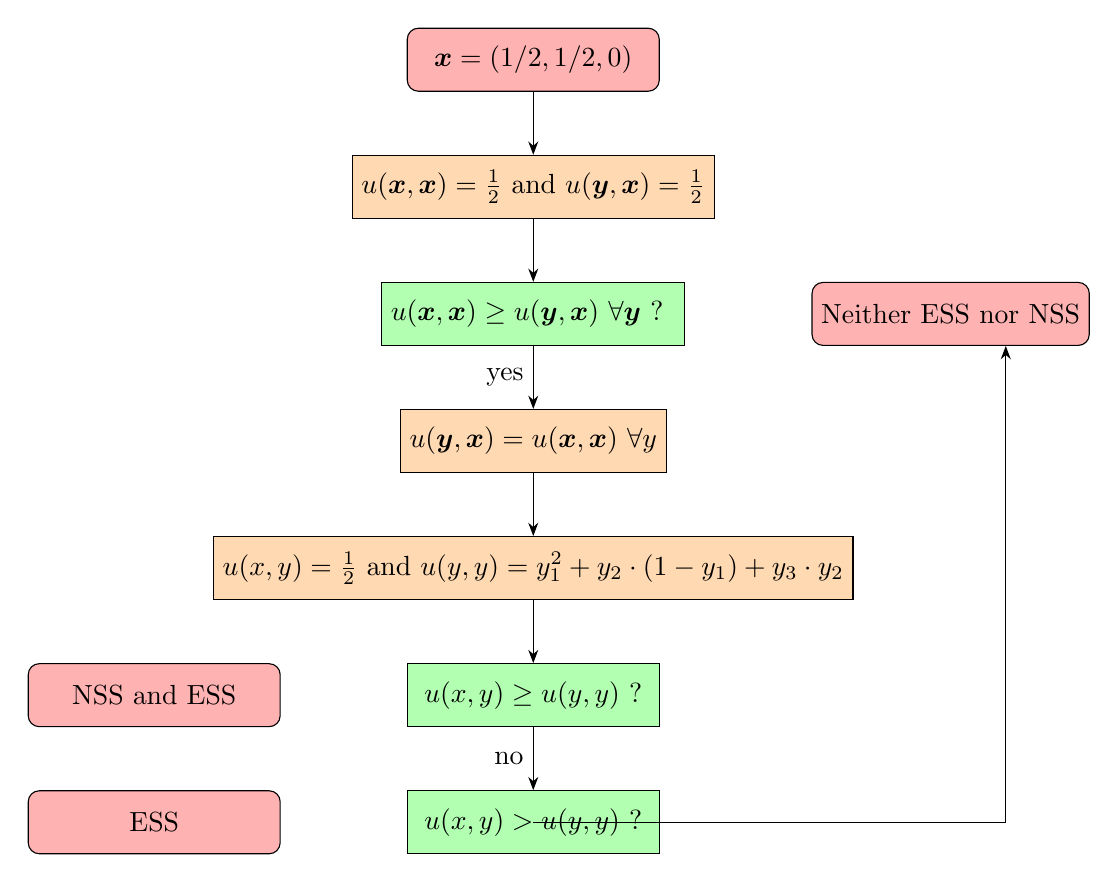
\begin{tikzpicture}[
            node distance = 8mm and 16mm,
            start chain = A going below,
            base/.style = {draw, minimum width=32mm, minimum height=8mm,
                    align=center, on chain=A},
            startstop/.style = {base, rectangle, rounded corners, fill=red!30},
            process/.style = {base, rectangle, fill=orange!30},
            decision/.style = {base, rectangle, fill=green!30},
            every edge quotes/.style = {auto=right}]

        \node [startstop]       {$\bm{x} = (1 / 2, 1/2, 0)$}; % A-1
        \node [process]         {$u(\bm{x}, \bm{x}) = \frac{1}{2}$ and $u(\bm{y}, \bm{x}) = \frac{1}{2}$}; % A-2
        \node [decision]        {$u(\bm{x}, \bm{x}) \geq u(\bm{y}, \bm{x}) \ \forall \bm{y}$ ? }; % A-3
        \node [process]         {$u(\bm{y}, \bm{x}) = u(\bm{x}, \bm{x}) \ \forall y$}; % A-4
        \node [process]         {$u(x, y) = \frac{1}{2}$ and $u(y, y) = y_1^2 + y_2 \cdot (1 - y_1) + y_3 \cdot y_2$}; % A-5
        \node [decision]        {$u(x, y) \geq u(y, y)$ ?}; % A-6
        \node [decision]        {$u(x, y) > u(y, y)$ ?}; % A-7

        % Out
        \node [startstop,
            right =of A-3]      {Neither ESS nor NSS}; % A-8
        \node [startstop,
            left =of A-6]      {NSS and ESS}; % A-9
        \node [startstop,
            left =of A-7]      {ESS}; % A-10
        %%
        \draw [arrows=-Stealth]
        (A-1) edge  (A-2)
        (A-2) edge (A-3)
        (A-3) edge["yes"] (A-4)
        (A-4) edge (A-5)
        (A-5) edge (A-6)
        (A-6) edge["no"] (A-7)
        (A-7) |- ($(A-7.east)!0.!(A-8.south)$)
        -|([xshift=7mm] A-8.south);
    \end{tikzpicture}
\end{center}

\subsubsection{Replicator dynamics}

Corner utilities are,

\begin{equation}
    u(\bm{e}^1, \bm{x}) = x_1, \ u(\bm{e}^2, \bm{x}) = (1 - x_1),\ u(\bm{e}^3, \bm{x}) = x_2
\end{equation}

\textbf{1. Fixed points}

The fixed points here are too complex, probably not there

\textbf{2. Boundaries}

Remember that $\sum_i \dot{x_i} = 0$ so on the boundaries one only needs to find one $x_i$.

\begin{itemize}
    \item $\bm{x} = \left( \alpha, 0, 1-\alpha \right)$ yields, $\dot{x}_1 = 1 - \alpha > 0$, we move towards $(1)$
    \item $\bm{x} = \left( 0, \alpha, 1-\alpha \right)$ yields $1 - 2\alpha + \alpha^2 > 0$, we move towards $(2)$
    \item $\bm{x} = \left( \alpha, 1-\alpha, 0 \right)$ yields $2 \alpha - 1 > 0 \iff \alpha > \frac{1}{2}$, we move away from the mid point.
\end{itemize}

\textbf{3. Bisector}

The only interesting bisector is the one were 1 and 2 are constant since the whole system moves towards 1 and 2. That is $\bm{x} = (\alpha, \alpha, 1 - 2\alpha)$.

Then we can compute,

\begin{equation}
    \begin{split}
        \dot{x}_1 &= \left( \alpha - \alpha^2 - \alpha \cdot (1 - \alpha) - \alpha + 2\alpha^2 \right) \alpha \\
        &= \alpha^2 \cdot (2 \alpha - 1) < 0 \\
        \dot{x}_2 &= \alpha \cdot (1 - \alpha) \cdot (1 - 2\alpha) > 0 \\
        \dot{x}_3 &= - (\dot{x}_1 + \dot{x}_2) = -\alpha \cdot (1 - 2\alpha)^2 < 0
    \end{split}
\end{equation}

When we are the bisector apart from the two edge points $\alpha = 0$ and $\alpha = \frac{1}{2}$ we are moving towards 2. This implies that the manifold is towards 1.

\begin{center}
    \includegraphics[width=0.5\textwidth]{images/weibull_14.PNG}
\end{center}

\end{document}
